\documentclass[conference]{IEEEtran}
\IEEEoverridecommandlockouts
% The preceding line is only needed to identify funding in the first footnote. If that is unneeded, please comment it out.
\usepackage{cite}
\usepackage{amsmath,amssymb,amsfonts}
\usepackage{algorithmic}
\usepackage{graphicx}
\usepackage{textcomp}
\usepackage{xcolor}
\def\BibTeX{{\rm B\kern-.05em{\sc i\kern-.025em b}\kern-.08em
    T\kern-.1667em\lower.7ex\hbox{E}\kern-.125emX}}
\begin{document}

\title{LOB-Based Price Movement Strategy}

\makeatletter
\newcommand{\linebreakand}{%
  \end{@IEEEauthorhalign}
  \hfill\mbox{}\par
  \mbox{}\hfill\begin{@IEEEauthorhalign}
}
\makeatother


\author{\IEEEauthorblockN{Shuoqi Zhang}
\IEEEauthorblockA{\textit{Department of Engineering Mathematics} \\
\textit{University of Bristol}\\
Bristol, United Kingdom \\
bt22161@bristol.ac.uk}
\and
\IEEEauthorblockN{Haolin Li}
\IEEEauthorblockA{\textit{Department of Engineering Mathematics} \\
\textit{University of Bristol}\\
Bristol, United Kingdom \\
ka23404@bristol.ac.uk}
\linebreakand %
\IEEEauthorblockN{Thanmai Gavini}
\IEEEauthorblockA{\textit{Department of Engineering Mathematics} \\
\textit{University of Bristol}\\
Bristol, United Kingdom \\
fc23722@bristol.ac.uk}
\and
\IEEEauthorblockN{Asad Hussain}
\IEEEauthorblockA{\textit{Department of Engineering Mathematics} \\
\textit{University of Bristol}\\
Bristol, United Kingdom \\
pi23794@bristol.ac.uk}
}

\maketitle

\begin{abstract}
There are three major simulation trading methods focusing on Limit Order Book (LOB) and tapes data which are explored in this study. Literature from relevant studies explores the evolution from traditional human analysis to the integration of neural networks particularly Convolutional Neural Networks (CNN) and Long Short-Term Memory (LSTM) models in stock trading prediction. The trading strategies include the simulation of Moving Average Strategy, price prediction for trading signals using ARIMA and LSTM models, and price movement prediction for trading signals through LSTM. The details of each strategy are explored including parameter identification, forecasting, and implementation. Furthermore, the study provides insights into the data description, preparation, and storage, emphasizing the importance of efficient data handling, visualization, and analysis techniques. The comparative performance of the strategies demonstrates the superiority of LSTM-based approaches, particularly in price prediction and movement analysis. The challenges encountered during back testing are focused upon, highlighting the need for dynamic order splitting to optimize trading outcomes. The study successfully compares models with complex data features being integrated. The developed trading strategies are robust and adapt to but also capitalize on the dynamic nature of financial markets. Code, data, and pretrained models are available online at https://github.com/UoB-DSMP-2023-24/dsmp-2024-group21.
\end{abstract}

\section{Introduction}
In this era of exponential data growth, finance markets can be considered as one of the prime examples of big data. These financial markets produce data that is rich in volume, variety and velocity, providing an opportunity to apply analytical techniques for actionable insights.

This project delves into Level-2 data analytics, which provides a more granular view of the bid-ask dynamics in the financial industry, like the Amazon shares, using the Limit Order Books (LOB). An LOB for a highly traded asset like Amazon can generate over 100,000 data points on an average day, each revealing detailed price and quantity pairings that reflect the trader behaviour and market sentiment.

The aim is to identify reliable trading signals for buy and sell decisions from the Level-2 data and convert the obtained insights into profitable trading strategies. The methodology holds various analytical techniques like the LSTM and the ARIMA models. The difficulty lies in not just processing the huge amounts of data but in deriving meaningful insights from this unpredictable market. The project aims to overcome these challenges through extensive data collation, data analysis and careful methodical testing. In addition, it aims to provide insights into the operational feasibility of the strategy by simulating trading scenarios with derivative signals.

The objectives are clear throughout this project, to develop a robust analytical framework that is capable of processing and analysing Level-2 data efficiently, identifying predictive patterns that are both statistically significant and economically impactful, and demonstrating that these potential strategies can generate profit in live trading scenarios in the long run.

\section{Literature Review}
Before proceeding to make trading decisions, multiple trading techniques and neural network models were studied in order to complete this project using relatively appropriate methods. The previous work mainly involved human analysis of stock movements to predict the rise or fall of the stock at the next point of time or time period, but there are certain limitations and imprecisions in the stock movements analyzed through human emotions \cite{b1}. 

Therefore, neural networks are introduced into the field of stock trading. Convolutional neural networks utilize large-scale limit order data to predict stock movements in the coming period. The model is fed with LOBs (both buy and sell data) and by evaluating and comparing the results with those of SVM and MLP techniques, it was found that in the short term, the convolutional neural network significantly outperforms the other two in terms of prediction \cite{b2}. 

A group of researchers collected Limit Order Book (LOB) data from Nasdaq from 2017 to 2019, used multivariate time series models to predict the LOB data, and proposed a labeling procedure to improve the feasibility of high-frequency trading strategies \cite{b11}.

Another article found that since stock price movements change with the timeline, which means that stock prices are time-based sequences, then the ARIMA model is effective in performing short-term price changes of stocks with minimal error, which can effectively help investors to formulate investment strategies \cite{b3}. A group of experimentalists obtained the stock price data of Chinese baijiu from Yahoo Finance website, which contains the opening price, closing price and maximum price of each day. The experimenters predicted the stock price by using different methods (LSTM, ARIMA, linear regression) and evaluated the results, in which the root mean square error (RMSE) of the LSTM model on the test set was 0.023, and the $R^2$ score was 0.89. By comparing the different results, it was found that the LSTM model was able to better capture the characteristics of the data changes over time \cite{b4}.

When developing trading strategies, a group of experimenters achieved moderate performance results by applying the LSTM model to basic investing; when using the LSTM model  with a basic leveraged trading strategy (holding cash when the predicted price of a stock is lower than the current price, and using leverage to buy and hold a stock when the predicted price is higher than or equal to the current price), the results of the experiment were very impressive (with significant increases in both Alpha and Beta values) \cite{b12}.  The experiments illustrate that when using a combination of LSTM models and trading strategies has great potential for investment.

In another study, the experimenters used a brand new method (CNN-LSTM model) to predict the stock market index. Convolutional neural network was used to extract features of prices from raw stock data and then output. The output of the convolutional neural network is used as an input to the LSTM, which better analyzes the future movement of the stock through its long-term memory capability. Experimental results show that CNN-LSTM approach performs well in predicting stock market indices \cite{b5}.


\section{Methodology}
This section elaborates on three simulation trading methods for LOBs and tapes data.

% \subsection{ARIMA model}
% The ARIMA is a widespread statistical approach for forecasting time series data. It has three components, they are:

% a) An Auto-regression (AR) model shows a changing variable in a time series that regresses on its own lagged or prior values. This component is dependant on the parameter (p) which represent the number of lag observations in the model, also known as the lag order \cite{b8}. 

% b) Integrated (I) component represents the differencing of raw observations, thus allowing the time series to become stationary. This is important because non-stationary data can produce unreliable or false results. This component is denoted by the parameter (d), the number of times the raw observations are differenced, also called as the degree of differencing \cite{b8}.

% c) The Moving average (MA) component uses past forecast errors in a regression-like model rather than using past values of the forecast variable in a regression. It is denoted by the parameter (q), which is the size of the moving average window, also known as the order of the moving average \cite{b9}.

% ARIMA (p, d, q) indicates an ARIMA model with "p" as the autoregressive component order, "d" as the degree of differencing needed to establish stationarity, and "q" as the moving average component order. The model's effectiveness depends on optimising p, d, and q parameters through repeated testing and validation against historical data \cite{b9}.

% The steps to implement the ARIMA methodology are \cite{b10}:

% a)	Model Identification
% The ARIMA model needs stationary time series data. Thus, data stationarity is assessed first. If data is not stationary, determine the degree of differencing needed to make it stationary.

% b)	Parameters Identification (ACF and PACF)
% For the ARIMA model to work, d (stationary data), q (residual lags), and p (previous data points) must be set correctly. Finding the right values of q and p requires the Autocorrelation Function (ACF) and Partial Autocorrelation Function (PACF). These account for all intermediate delays to estimate the correlation between the series' present value and its prior values.

% c)	Selecting the Best ARIMA Model
% After discovering stationarity data transformations and parameters using ACF and PACF analysis, different ARIMA models may be examined. Next, estimate autoregressive parameters and choose the best model.

% d)	Forecasting
% Selecting the best model lets you predict future values. In many situations, ARIMA forecasting is more accurate than other time series forecasting approaches.

% Below is the mathematical representation of the ARIMA model:

% \[
% (1 - \sum_{i=1}^p \phi_i L^i) (1 - L)^d X_t = (1 + \sum_{j=1}^q \theta_j L^j) \epsilon_t
% \]

% Where:
% \begin{itemize}
%     \item $X_t$ is the time series data.
%     \item $L$ is the lag operator (i.e., $LX_t = X_{t-1}$).
%     \item $d$ is the order of differencing required to make the series stationary.
%     \item $p$ is the number of lag observations included in the model (autoregressive terms).
%     \item $q$ is the number of lagged forecast errors in the prediction equation (moving average terms).
%     \item $\phi_1, \phi_2, ..., \phi_p$ are the parameters of the autoregressive part of the model.
%     \item $\theta_1, \theta_2, ..., \theta_q$ are the parameters of the moving average part.
%     \item $\epsilon_t$ is white noise error terms.
% \end{itemize}


\subsection{Simulation of Moving Average Strategy}


The moving average strategy is designed to capitalise on long and short positions in the market. The aim is to assess the effectiveness of the strategy under different market conditions, and in particular to check how the variation of limit orders (LOBs) thickness affects the strategy performance.

A simple moving average (SMA), is calculated by taking the arithmetic mean of a given set of values over a specified period. 
% \begin{equation}
% \text{SMA}= \frac{1}{n}\sum_{i=1}^{n} A_i
% \end{equation}
% where $n$ is the number of time period and  $A_i$ is the average in period $i$.

A moving average strategy involves using simple moving averages to generate trading signals. Buying begins when the short-term moving average crosses the long-term moving average upwards, and selling begins when the short-term average crosses the long-term average downwards.

When there is a trading signal, the algorithm will start a trade with a risk ratio decided by Average True Range (ATR). Calculation of stop-loss and take-profit points by risk ratio and current price. Based on the signal, the algorithm executes a market order for the traded amount based on the current LOB data. The position is then monitored for a period of time and closed when the specified stop-loss and take-profit points are reached.

During the simulations, it was discovered that when the LOB was not sufficiently deep, the strategy often failed to execute trades at the intended prices, leading to slippage and unanticipated losses. This issue was addressed by:
The strategy was fine-tuned to modify these points in response to the observed LOB depth, allowing for tighter controls under thin LOB conditions. For thinner books, larger buffers were introduced to accommodate price volatility and slippage.

\subsection{Price Prediction for Trading Signals}
While the moving average strategy captures price trends through simple statistical measures, more complex financial trading data often require advanced models to extract key information. Predicting future prices using historical data allows generating trading signals by comparing these predictions with current prices. In this project, two time-series forecasting methods were utilized, and performance was compared in Section \ref{section4}.

\subsubsection{ARIMA Price Prediction}

The ARIMA\cite{b8,b9,b10} model captures the dynamics of price movements through its components: auto-regression (AR), integration (I), and moving averages (MA). An Auto-regression (AR) model shows a changing variable in a time series that regresses on its own lagged or prior values. Integrated (I) component represents the differencing of raw observations, thus allowing the time series to become stationary. The Moving Average (MA) component uses past forecast errors in a regression-like model rather than using past values of the forecast variable in a regression.  $\text{ARIMA}  (p, d, q)$ indicates an ARIMA model with $p$ as the autoregressive component order, $d$ as the degree of differencing needed to establish stationarity, and $q$ as the moving average component order. The model's effectiveness depends on optimising $p$, $d$, and $q$ parameters through repeated testing and validation against historical data.

Below is the mathematical representation of the ARIMA model:

\[
(1 - \sum_{i=1}^p \phi_i L^i) (1 - L)^d X_t = (1 + \sum_{j=1}^q \theta_j L^j) \epsilon_t
\]

Where:
\begin{itemize}
    \item $X_t$ is the time series data.
    \item $L$ is the lag operator (i.e., $LX_t = X_{t-1}$).
    \item $d$ is the order of differencing required to make the series stationary.
    \item $p$ is the number of lag observations included in the model (autoregressive terms).
    \item $q$ is the number of lagged forecast errors in the prediction equation (moving average terms).
    \item $\phi_1, \phi_2, ..., \phi_p$ are the parameters of the autoregressive part of the model.
    \item $\theta_1, \theta_2, ..., \theta_q$ are the parameters of the moving average part.
    \item $\epsilon_t$ is white noise error terms.
\end{itemize}

To implement the ARIMA methodology, data stationarity is assessed first. If data is not stationary, determine the degree of differencing needed to make it stationary. For the ARIMA model to work, d (stationary data), q (residual lags), and p (previous data points) must be set correctly. Finding the right values of q and p requires the Autocorrelation Function (ACF) and Partial Autocorrelation Function (PACF). Next, estimate autoregressive parameters and choose the best model. Selecting the best model lets you predict future values. 



\subsubsection{LSTM Price Prediction} 

Conversely, the LSTM (Long Short-Term Memory) model excels in handling complex patterns that involve long-term dependencies in time series data. Unlike traditional models that may struggle with the volatility of financial markets, LSTM can learn from a broader context within the data sequence. LSTM has several repeating modules update the hidden state. Each repeated module in LSTM contains three sigmoid layers and one tanh layer, which interact with each other and each time they can control the output content of the next step \cite{b6}. Each LSTM storage cell consists of three gates. Input gates control the input information within the new cell including the output information from the previous cell. The forget gate filters the information and decides which information needs to be discarded. Output gates, on the other hand, control the output information to the next cell. In these gates, zero means that no information is run through and 1 means that all information is run through. This ensures that the network learns the information that needs to be memorized, and discards the information that is not needed.

\begin{figure}[tb]
\centerline{\includegraphics[scale=0.45]{LSTM1.png}}
\caption{LSTM model \cite{b6}}
\label{fig}
\end{figure}
\subsubsection{Limitations} 

While ARIMA, LSTM provide rolling predictions that closely match actual price movements with metrics such as mean squared error (MSE), these models may not fully capture the real market price dynamically. These models primarily rely on historical price data to forecast future prices. By adding some noise to the previous data, a prediction can be achieved with minimal loss on their part. This approach, although statistically valid, essentially results in forecasts that are flat versions of historical price curves.

The generated forecasts are similar to an enhanced version of the moving average model. Although this method smooths out price fluctuations and provides a clearer trend line, it significantly limits the model’s capability to extract and leverage new market information. The stock prices are not the result of a couple of underlying causal factors, but a rather a multitude of contributions as well as a good dose of human irrationality. As a result, price forecasting models may not provide substantial improvements in understanding or responding to new market conditions that are not directly reflected in past data.


\subsection{Price Movement Prediction for Trading Signals}
The limitations of price forecasting models underscore the need to integrate other data types or use more sophisticated analytical techniques that can incorporate external factors affecting the market. By doing this, forecasting models may provide more insightful predictions that better reflect underlying market dynamics, rather than merely repeating past trends with minor modifications.

Given the limitations of traditional price forecasting models, the approach consists of designing a forecasting model that focuses on price changes rather than absolute prices. This model uses an LSTM as its core network but modifies its output to predict changes in price, which helps circumvent the systemic lags encountered when predicting absolute prices.

To enhance the model’s universality and robustness, the model incorporates various technical indicators as input features. These include:
\begin{enumerate}    
  \item Relative Strength Index (RSI): This measures the velocity and magnitude of directional price movements and provides insights into overbought or oversold conditions. For our model, RSI is calculated over a 15-day period.
  \item Exponential Moving Averages (EMAs): These are used to smooth out price data and better identify trends by giving more weight to recent prices. EMAs are calculated for different time spans like 20, 100, and 150 time period to capture short-term, medium-term, and long-term trends. 
  \item Best Bid and Ask Prices: These are calculated from limit order book. They are the lowest ask and highest bid in one certain moment.These elements are crucial for understanding the immediate market conditions and potential order positions. 
  \item Market Depth: Use current ask/bid orders to calculate the depth of each sides of trade, as an indicator of the liquidity of the market, showing how quickly and at what volume transactions can be executed without significantly impacting the market price.
\end{enumerate}

There are also some factors help us in trading time decision. The target variable is constructed as the difference between the closing and opening prices, shifted by one period to predict future changes:
\[ \text{Target}_t = \text{Close}_t - \text{Open}_t \]
\[ \text{Target}_{t+1} = \text{Target}_t \]

Additionally, a classification target is created to indicate whether the price is expected to increase (1) or decrease (0):
\[ \text{TargetClass}_t = 
   \begin{cases} 
   1 & \text{if } \text{Target}_{t+1} > 0 \\
   0 & \text{otherwise}
   \end{cases}
\]

Finally, anticipating future closing prices based on adjusted close prices:
\[ \text{TargetNextClose}_t = \text{Close}_{t+1} \]

By predicting price changes rather than absolute prices and integrating a broader set of market and technical indicators, this revised model aims to provide more actionable insights for trading strategies. This methodology not only addresses the inherent lags found in previous models but also improves adaptability to new market dynamics, potentially enhancing predictive accuracy and trading outcomes.

\section{Data Description / Preparation}

Our project utilizes actual trading data from both tapes and the Limit Order Book (LOB) for a specific stock, covering the period from January 2, 2025, to July 1, 2025. The data comprises detailed transaction logs and order book entries capturing the market dynamics over the specified period.

\subsection{Data Prepossessing}

To facilitate trading simulations, the data underwent a prepossessing phase:
\begin{enumerate}    
  \item LOB Data: Only relevant data fields such as timestamps, types, and all orders associated with these timestamps were retained.The timestamps were merged with their respective dates to create new datetime indices. Ask and bid orders were separated; each order, containing price and quantity, was organized either in ascending or descending order based on price. 
  \item Tapes Data: Similar to LOB data, timestamps were combined with dates to form new datetime indices. Each row includes the datetime index, price, and quantity of transactions at that specific time. 
  
\end{enumerate}


To enhance the manageability and relevance of the LOB and tapes data for analysis and simulation, the data was resampled on a per-second basis. This approach was taken to reduce data redundancy and focus on the most relevant market conditions at each discrete second. 

For LOB data, we need a Ask-Bid snapshot at the given second. Among the multitude of orders received within any given second, only the orders at the timestamp closest to the rounded up second were selected. 

For tapes data, we also retain they last row closest to the rounded up seconds. We calculate the open, close, high and low price for indicators computation.



\subsection{Data Storage}

Given the large volume of data involved, efficient data retrieval was a critical concern. This project employed the HDF5 format for data storage due to its storage and read efficiency. HDF5 provides a robust framework for handling large datasets by allowing data to be stored in a compressed, binary format which enhances read/write efficiency. Table ~\ref{hdf5} shows the comparison between HDF5 and CSV file format on file size and reading time. It turns out HDF5 have better performance on both indicators. 

\begin{table}[tb]
\caption{HDF5 and CSV comparison}
\begin{center}
\begin{tabular}{|p{0.2\columnwidth}|p{0.2\columnwidth}|p{0.2\columnwidth}|}
\hline
\textbf{File Format} & \textbf{File Size} & \textbf{Reading Time} \\
\hline
HDF5 & \textbf{2.81 GB} &  \textbf{57 second}\\
\hline
CSV & 7.75 GB & 11 minute\\
\hline
\end{tabular}
\label{hdf5}
\end{center}
\end{table}


The use of HDF5 not only significantly reduced the data loading time but also facilitated more complex data analyses without the performance bottlenecks typically associated with large datasets. This enhanced data handling capability is crucial for conducting high-frequency trading simulations where speed and data integrity are paramount. When saving processed data, we use batching techniques to save data more efficiently by reducing the I/O overhead and making better use of memory. 

\subsection{Data Visualization}
After processing the data, we employed several data visualization techniques to assist in analyzing the data and formulating trading strategies.
\subsubsection{Candlestick Line}
Candlestick Charts, also known as K-line charts, are a type of financial chart used to display the price dynamics of financial assets. They primarily utilize transaction data points: Open, High, Low, and Close (OHLC). These charts provide a visual summary of price actions, aiding market participants in making informed trading decisions. In this project, the candlestick charts are drawn based on the prepossessed OHLC values from the tapes data. This data allows us to capture the price fluctuations for each trading day or session, thereby analyzing market trends and volatility.

\begin{figure}[tb]
    \centerline{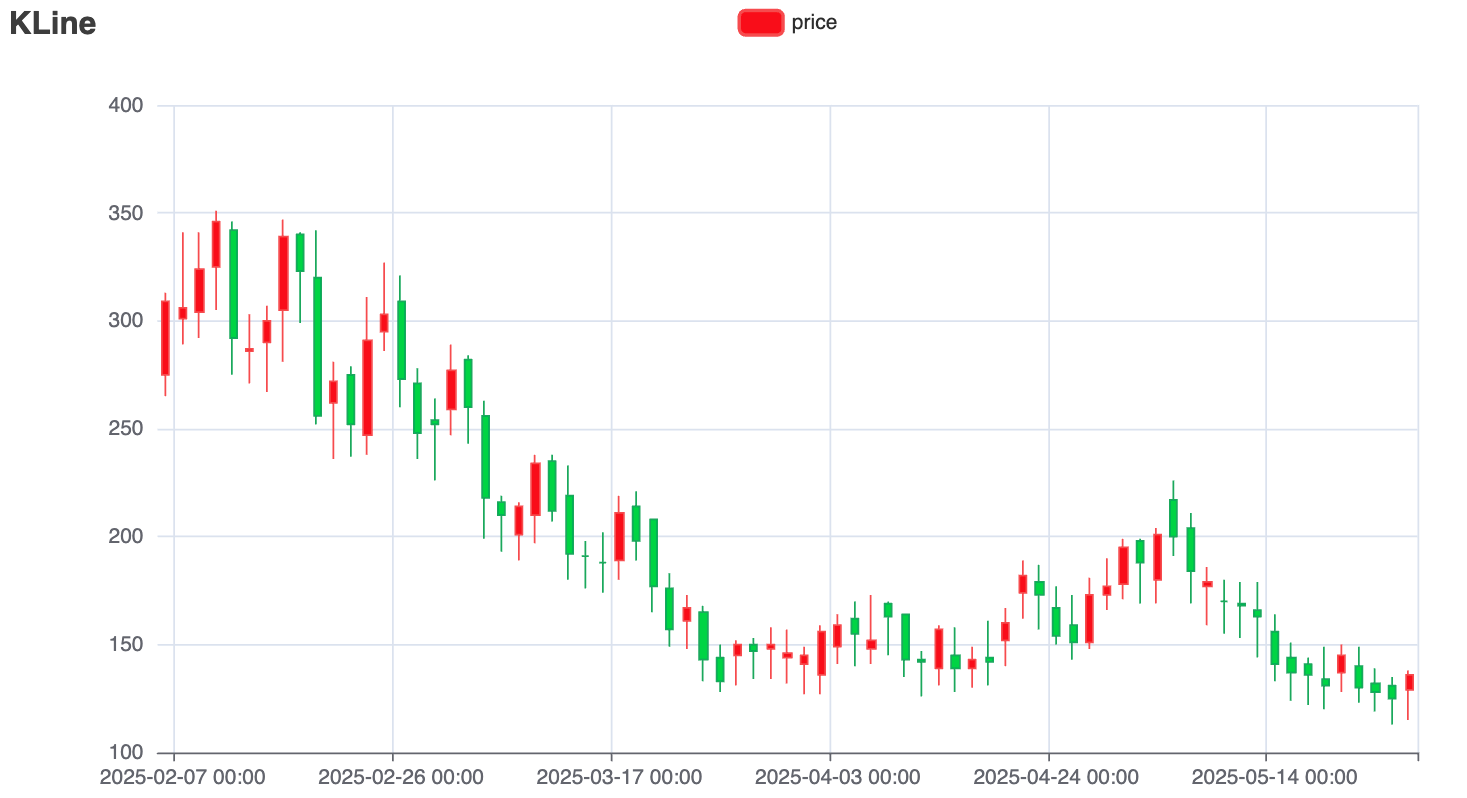
\includegraphics[width=0.5\textwidth]{Kline.png}}
    \caption{Kline}
    \label{Kline.png}
\end{figure}


Candlestick charts reveal several key pieces of information:
\begin{enumerate}    
  \item Price Volatility: The body and wicks of the candlesticks show the range of price movements within a certain period.
  \item Market Trends: The direction and color of the candlesticks can indicate the overall trend—whether the market is trending upward or downward.
  \item Support and Resistance Levels: Continuous formations in the candlestick patterns can help identify potential support and resistance levels, which are crucial for setting entry points and stop-loss levels.

\end{enumerate}



\subsubsection{Depth Chart}

Following the analysis using candlestick charts, we further explore depth charts, another critical visualization tool derived from Limit Order Book (LOB) data. Depth charts offer a graphical representation of the buying and selling pressure in the market by displaying the quantity of buy and sell orders at different price levels.
\begin{figure}[tb]
    \centerline{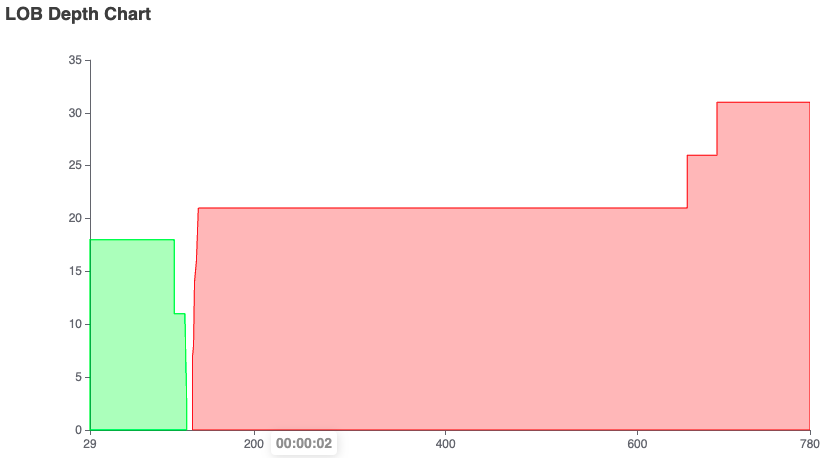
\includegraphics[width=0.5\textwidth]{depthchart.png}}
    \caption{Depth Chart}
    \label{depthchart}
\end{figure}
Depth charts are constructed from LOB data, which contains detailed information about buy and sell orders at various price points. These charts shows the demand and supply in the market, helping traders understand the potential price movements and market depth at a glance. We
make a animation by play depth charts one by one and it is a better way to observe the market movement.

To enhance the analysis, the depth charts are integrated with tapes data, which records actual transactions. This integration provides a dynamic view of the market, combining the theoretical orders with actual market executions, and allows traders to observe how transactions affect the LOB in real-time.

 By observing the depth of buy and sell orders, traders can estimate the liquidity of the market. A deep market with large orders at multiple price levels typically indicates higher liquidity, suggesting that large transactions can be executed without significantly impacting the price. It can also reveal natural price support and resistance levels, where large concentrations of buy or sell orders are placed.


\subsubsection{Backtesting Visualization}

In addition to employing various data visualization techniques for analyzing market data, our study has also developed a dedicated visualization module for the simulation of trading strategies during backtesting. This module enhances our ability to assess the effectiveness of different trading strategies by visually representing their dynamics.
\begin{figure*}[tb]
    \centerline{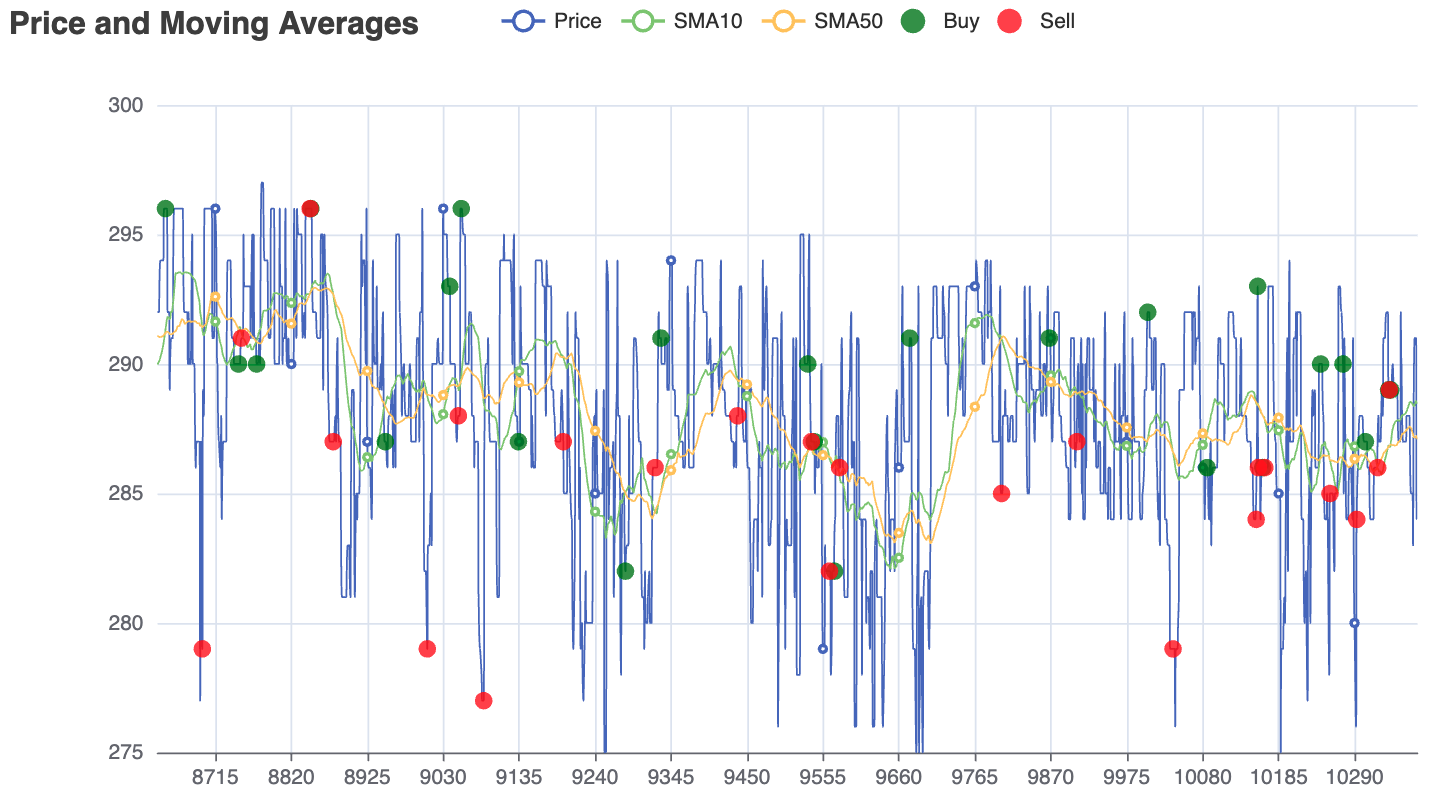
\includegraphics[width=\textwidth]{backtesting.png}}
    \caption{Backtesting Visualization}
    \label{backtesting}
\end{figure*}

The visualization module is designed to display price charts over different sampling periods, allowing for a comprehensive temporal analysis of price movements. On the same chart, the module allows for the display of various trading factors and the positions of trading signals. This integration helps in correlating specific market events or conditions with the corresponding trading actions.


\section{Results and Discussion} \label{section4}

This section elaborates on several experiments and also discusses the insights and challenges we faced.
\subsection{Price Predict Experiment}
An experiment between ARIMA and LSTM price prediction model was designed, aiming to evaluate and compare the efficiency of each model in the context of financial time-series forecasting.

Using previous predictions as new input to predict a few more steps, the results differ significantly from the original. This is due to the fact that the error per prediction is cumulative. Hence, both models utilize a sliding window to rolling forecast.


The overall prediction accuracy of each model was assessed by measuring cumulative errors using mean absolute error (MAE) and mean squared error (MSE) over the test period. TABLE~\ref{price} shows the results.
 
 \begin{table}[tb]
\caption{ARIMA and LSTM comparison}
\begin{center}
\begin{tabular}{|p{0.2\columnwidth}|p{0.2\columnwidth}|p{0.2\columnwidth}|}
\hline
\textbf{File Format} & \textbf{MSE} & \textbf{MAE} \\
\hline
LSTM & \textbf{0.0109} &  \textbf{0.0084}\\
\hline
ARIMA & 0.0357 & 0.0146\\
\hline
\end{tabular}
\label{price}
\end{center}
\end{table}

The LSTM model excels in capturing complex, non-linear patterns within the data patterns that are typically challenging for ARIMA models. This capability makes LSTM highly suitable for stock price forecasting, where the data often exhibits non-linear behaviors that simple statistical models would struggle to process. On the other hand, the ARIMA model performs well with linear relationships and seasonal patterns. While these attributes are beneficial for many forecasting scenarios, ARIMA's inability to adequately model the non-linear complexities required in stock price predictions can be a significant limitation.

The training time for ARIMA models is generally shorter due to its reliance on classical statistical methods for estimating model parameters. These parameters are fewer in number compared to those in deep learning models like LSTM, which translates to lower computational complexity. Consequently, the inference time for ARIMA is also relatively short, as the model involves straightforward mathematical calculations once the parameters are estimated. This simplicity and speed can be advantageous in applications where model complexity and training costs need to be minimized.

In summary, LSTM has better performance, although it takes more memory and time to train. As such, for the latter experiment the LSTM price prediction model is used to generate trading signals.


\subsection{SMA Backtesting}
The backtesting simulation needs to initialize several hyper parameters. The initial capital is the amount of capital in a virtual account. Then  a risk ratio is required to manage potential loss proportion per trade. The two parameters decide the maximum amount ordered per trade. A profit-loss ratio must be set for when a signal triggers a new trade. The profit-loss ratio is critical in deciding the threshold for taking profits and cutting losses. 

Another important hyper parameter is the average time span. Through Figure.~\ref{backtesting} the high volatility of price can be seen. When trading, it's necessary to remove those interruptions. One technique is with a longer time span, the average line is more smooth, which will produce less trade signals. Another way is to use bigger profit-loss zone, with the potential high risk. The profit-loss zone is calculated from the product of profit-loss ratio and average true range (ATR). Adding an ATR factor can directly control the zone area. So this experiment utilises several hyper parameter combination to find a profitable strategy setting. Calculate the profit rate to evaluate strategy performance.

\begin{table}[tb]
\caption{SMA experiment}
\begin{center}
\begin{tabular}{|p{0.2\columnwidth}|p{0.2\columnwidth}|p{0.2\columnwidth}|}
\hline
\textbf{ATR Factor} & \textbf{Time Span} & \textbf{Profit Rate} \\
\hline
 0.8 & 60 &  -0.143\\
\hline
 0.2 & 60 &  -0.004\\
\hline
 0.5 & 100 &  0.085\\
\hline
 0.5 & 20 &  -0.158\\
\hline
 \textbf{0.5} & \textbf{60} &  \textbf{0.184}\\
\hline
\end{tabular}
\label{SMA}
\end{center}
\end{table}


From Table~\ref{SMA}, it is evident that the ATR factor and the chosen time span significantly influence profitability. A larger ATR factor creates a wider profit-loss zone, which inherently carries a higher risk of substantial losses, potentially leading to a negative profit rate. Conversely, a smaller ATR factor indicates a more conservative strategy, typically characterized by not holding positions for long, which may limit potential losses but also constrain profit opportunities. Additionally, a larger time span reduces the frequency of trade signals, which can lead to a decrease in profit rate. On the other hand, a smaller time span may increase the risk of misinterpreting trading signals, which is also detrimental to performance.

\subsection{Price Movement LSTM Backtesting}
This section explores the Price Movement Model, which enhances trading strategies by generating signals based on predicted changes in price movement. Unlike traditional models that solely rely on tapes price, this innovative model integrates the analysis of LOB (Limit Order Book) depth to optimize both the timing and volume of trade executions.


The Price Movement Model takes several traditional stock indicators and limit order book as input feature, using historical data and current market conditions to forecast likely increases or decreases in price. When these predictions exceed certain predefined thresholds, trading signals are generated to indicate when to buy or sell.

\begin{table}[tb]
\caption{Strategy Performance }
\begin{center}
\begin{tabular}{|p{0.4\columnwidth}|p{0.2\columnwidth}|}
\hline
\textbf{Strategy Name} & \textbf{Profit Rate} \\
\hline
Simple Moving Average& 0.184 \\
\hline
LSTM Price Predict& 0.203 \\
\hline
LSTM Price Movement& \textbf{0.235} \\

\hline
\end{tabular}
\label{all}
\end{center}
\end{table}

We designed an experiment to test three strategies we mentioned above in their best parameter. TABLE~\ref{all} shows the different profit rate results on given tapes and LOB data. It can be found that LSTM price movement strategy has a significant increase in profitability compared to the other two strategies.

This may be due to the fact that the strategy learns more deeply about the information implicit in the markets. All the order data in the LOB and its changes over time contain an implied state that tapes data fails to characterize. A common approach to trading strategies is to find resistance and support levels where there is always a large number of trades making the trend flip at that location, which is a hidden message in stock price volatility. By analyzing the LOB data, we can more directly observe the change in the number of orders at different prices and find out the support level. Hidden states in LSTM networks can help refine the information to give estimates closer to the true price.

\subsection{Challenges}

During the backtesting of the above strategies, many difficulties were encountered. The most challenging of them, which is also instructive for a deeper understanding of the trade, is described below. 

\begin{table}[tb]
\caption{Order Split}
\begin{center}
\begin{tabular}{|p{0.2\columnwidth}|p{0.2\columnwidth}|p{0.15\columnwidth}|p{0.2\columnwidth}|}
\hline
\textbf{Total Amount} & \textbf{Use Order Split} & \textbf{Profit} & \textbf{Profit Rate}\\
\hline
2000 & no &  230& 0.115\\
\hline
4000 & no &  328& 0.082\\
\hline
6000 & no &  -402&  -0.067\\
\hline
2000 & yes &  222& 0.111\\
\hline
4000 & yes &  424& 0.106\\
\hline
6000 & yes &  552&  0.092\\
\hline
\end{tabular}
\label{lobdepth}
\end{center}
\end{table}

The problem is few LOB orders leading to a large discrepancy between the traded price and the expected price of some orders. As shown in Figure.~\ref{depthchart}, the number of ASK orders near the mid-price is very small, and the rest of the orders have a large difference from the mid-price. If the purchase quantity is large, it is easy to buy a large number of orders at a high price. There are two ways to solve this problem, one is to reduce the total amount of a single trade, which also reduces the share of each trade and makes it easier to close near the middle price. However, such a trading strategy has an immediate limit on the amount of trades, and even if you get a high profit rate you don't get a very high return. At the same time, due to the scarcity of the quantity of trades per transaction, much of the same suitable trading time is missed. The other is through the depth of the LOB order, dynamic split to adjust the number of orders, a small number of times in batches to complete the sale of the order. This can also be done at a price close to the mid-price, while the limitations on the number of shares traded are greatly reduced. We compared the total amount of different single transactions and whether to use dynamic order splitting yield and return, the results are shown in Table~\ref{lobdepth}. It can be seen that the use of dynamic order splitting guarantees the profit rate and also reduces the limitations on the total amount of trades.




\section{Further Work and Improvement}

To further improve this project, we could utilise LSTM for swing trading. Implementing LSTM models to predict not on price or price movement but on volatility will significant improve model performance in highly volatile and fluctuating stock market. By forecasting the degree and frequency of price fluctuations, model can give better entry and exit points, maximizing profits from market volatility.

Another area of further work would be optimizing stop-loss and take-profit points with LOB Data. Leveraging detailed LOB data to refine stop-loss and take-profit settings which would offer a strategic advantage. This approach allows for dynamically adjusting these thresholds based on real-time market depth and order flow, potentially increasing the accuracy and effectiveness of these critical parameters.

Furthermore, by identifying support and resistance levels with refined strategies, better strategic decisions in both entry and exit phases could be facilitated. Developing strategies that more accurately identify support and resistance levels can lead to the creation of more robust trading systems which would also increase the quality of this project. These strategies could incorporate advanced analytics to identify these levels more precisely.

Lastly, exploring medium to long-term operational strategies could improve returns. There is substantial potential in exploring longer-term holding strategies that capitalize on larger market movements. These strategies would involve holding positions over extended periods to benefit from significant price differentials.







\section{Conclusion}
This project entailed the design and extensive testing of three distinct trading strategies. The moving average strategy was established as the baseline for comparison, with a specific focus on exploring the impacts of the Average True Range (ATR) factor and time span on model profitability.

For price prediction, we employed both ARIMA and LSTM models to evaluate and contrast their performance capabilities. Through these comparative analyses, the LSTM model emerged as the superior choice for our final price prediction strategy, offering a noticeable improvement over the baseline moving average strategy. This selection was based on LSTM's enhanced ability to capture complex patterns and trends in price movements, which ARIMA struggled with.

Furthermore, the project integrated multiple features, especially leveraging LOB (Limit Order Book) data characteristics, into a price movement model. This advanced model significantly improved our understanding of market depth and liquidity. Compared to the earlier models, this approach resulted in a substantial increase in profitability, demonstrating the value of incorporating comprehensive market data features into trading strategies.

By systematically comparing these models and integrating complex data features, our project has successfully developed robust trading strategies that not only adapt but also capitalize on the dynamic nature of financial markets, resulting in enhanced profitability and strategic advantage.


\begin{thebibliography}{00}
\bibitem{b1} Z. Chang and Z. Zhang, "Judging Stock Trends According to the Sentiments of Stock Comments in Expert Forums," Electronics, vol. 12, no. 722, 2023.
\bibitem{b2} A. Tsantekidis, N. Passalis, A. Tefas, J. Kanniainen, M. Gabbouj, and A. Iosifidis, "Forecasting Stock Prices from the Limit Order Book using Convolutional Neural Networks," 2017 IEEE 19th Conference on Business Informatics, pp. 7-10, doi: 10.1109/CBI.2017.23.
\bibitem{b3} A. A. Adebiyi, A. O. Adewumi, and C. K. Ayo, "Stock Price Prediction Using the ARIMA Model," University of KwaZulu-Natal and Covenant University.
\bibitem{b4} J. Li, "Predicting Stock Prices of Chinese Liquor Companies with the LSTM Network: A Case Study on Shede Spirits," in Highlights in Science, Engineering and Technology AIDML 2023, vol. 57, 2023, pp. 180-183, Department of Computer Science, Michigan State University
\bibitem{b5} H. Song and H. Choi, "Forecasting Stock Market Indices Using the Recurrent Neural Network Based Hybrid Models: CNN-LSTM, GRU-CNN, and Ensemble Models," Appl. Sci., vol. 13, no. 4644, 2023.
\bibitem{b6} R. Zhang, C. Huang, W. Zhang, and S. Chen, "Multi Factor Stock Selection Model Based on LSTM," International Journal of Economics and Finance, vol. 10, no. 8, p. 36, Jun. 2018.
\bibitem{b7} A. Ceni, "Random Orthogonal Additive Filters: A Solution to the Vanishing/Exploding Gradient of Deep Neural Networks," 2022.
\bibitem{b8} A. Hayes, “Autoregressive Integrated Moving Average (ARIMA) Prediction Model,” Investopedia, Feb. 23, 2024. Available: https://www.investopedia.com/terms/a/autoregressive-integrated-moving-average-arima.asp#toc-arima-parameters
\bibitem{b9} R. J. Hyndman and G. Athanasopoulos, Forecasting : Principles and Practice, 2nd ed. Heathmont, Vic.: Otexts, 2018. Available: https://otexts.com/fpp2/
\bibitem{b10} George, G. M. Jenkins, and G. C. Reinsel, Time Series Analysis. 1994.
\bibitem{b11} A. Briola, S. Bartolucci, and T. Aste, "Deep Limit Order Book Forecasting," arXiv preprint arXiv:2403.09267, 2024.
\bibitem{b12} B. Wang and X. Zhang, "Deep Learning Applying on Stock Trading," Stanford University, CS230: Deep Learning Projects Spring 2021. 
\end{thebibliography}

\end{document}
